\section{Exact Oracles in Directed Planar Graphs}\label{exactPlanar}

Previous works have given exact distance oracles for directed planar graphs of size
$O(n^{5/3})$ with query time $O(\lg n)$ \cite{cohen2017fast}. This was improved recently
to use $O(n^{3/2})$ space \cite{gawrychowski2017better}. In the general case, we have
bounds that depend on the number of vertices $n$. But in the vertex-labeled case, we can
sometimes win space or obtain better query times by depending on the number of labels $\ell$.

\subsection{A distance oracle depending on $\ell$}
We cannot directly adapt the approach used in \cite{cohen2017fast} and \cite{gawrychowski2017better} to work
for the vertex-labeled case as it requires us to know the "target" vertex. However,
depending on $\ell$, we can use the $r$-division alone to show the following:
\begin{thm}\label{thm1}
  There is a distance oracle with space $O(n\ell^{2/3)})$, query time $O(\ell^{1/3})$ and
  preprocessing time $O(n^2/\ell^{1/3})$.
\end{thm}
\textit{Data structure}. Given a directed graph $G$, with nonnegative edge lengths and a number of labels $\ell$, we
construct an $r$-division. Remember, we use the $r$-division described in
\cite{klein2013structured}, which guarantees a constant number of holes in each region
and ensures the total number of boundary vertices is $O(n/\sqrt{r})$. Each region $R$ then has at most $r$ nodes and $O(\sqrt{r})$
boundary nodes. For each boundary node $u$, we store the shortest distance $d(u,\lambda)$
for all $\lambda \in L$ in a hash table. For all nodes inside $R$, we store the shortest
distance to all
boundary nodes as well as the distance to all labels present in $R$ in a hash table. \\
\\
\indent \textit{Query}. Given the query $Q(v, \lambda)$, if $v$ is a boundary node, we can look
up the distance in the hash table for $v$. If $v$ is not a boundary node, look up the
distances $\delta(u,v)+\delta(u,\lambda)$ for all boundary nodes $u$ and the distance
$\delta(v,\lambda)$ stored in the hash table for $v$ and return the minimum.

\subsubsection{Analysis}
\textbf{Preprocessing}. The $r$-division can be constructed in $O(n)$ time \cite{klein2013structured}. We then
construct a dense distance graph, that is, we construct the graph where each edge $uv\in
E$ has weight equal to $\delta(u,v)$ and $u$ and $v$ are both boundary nodes. We use
Klein's multiple source shortest path algorithm \cite{klein2005multiple} to compute DDG's
for each region of an $r$-division. For each region $R$ with $r$ nodes, we use $O(r\lg
r)$ preprocessing to compute distances $\delta(u,v)$ in $O(\lg r)$ time where either $u$
or $v$ is a boundary node. Since each region has $O(\sqrt{r})$ boundary nodes and $O(1)$
holes, we can compute all distances in $O(r\lg r)$ time. Since there are $O(n/r)$
regions, this yields a total running time of $O(nr\lg r/r)=O(n\lg r)$ to construct the
dense distance graph. We need to store distances from all boundary nodes to (potentially)
all other nodes in the graph. Henzinger et al. \cite{henzinger1997faster} gave a $O(n)$
time algorithm for single source shortest path in planar graphs. Using this for all
boundary nodes takes $O(n^2/\sqrt{r})$. To compute distances in the interior of each
region, we use Fredman and Tarjan's version of Djikstra's algorithm using Fibonacci heaps
\cite{fredman1987fibonacci}. This requires $O(n\lg n + m)$ time for each node. Each
region has $r$ vertices, the dense distance graph for the boundary nodes in the region has
$O(r)$ edges and the interior is a planar graph, so it has $O(r)$ edges as well. Using
this implementation for each node gives us a total running time of $O(r(r\lg r + r))=O(r^2\lg
r)$. The total preprocessing thus requires $O(n^2/\sqrt{r}+r^2\lg r)$ time. \\
\\
\textbf{Space}. For each boundary node, we store the distance to all labels. The $r$-division gives us
$O(n/r)$ regions and ensures we
get $O(\sqrt{r})$ boundary nodes, so this yields
$O(\frac{n}{r}\sqrt{r}\ell)=O(\frac{n}{\sqrt{r}}\ell)$ space. For all other nodes, we
store the distances to all boundary nodes and to all labels within that region. This
gives us $O(nr)$ space as we can potentially store the distances to all vertices in a
region $R$. This gives us a total of $O(\frac{n}{\sqrt{r}}\ell+nr)$ space. \\
\\
\textbf{Query}. The query $Q(u,\lambda)$ for a boundary node $u$ can be looked up in its hash table in
$O(1)$ time. For the query $Q(v,\lambda)$ for a vertex $v$ not on the boundary, we have
to find the minimum distance to $\lambda$ between all boundary nodes even if it exists in
that region as we are not guaranteed that the closest $\lambda$-labaled node is in the
region of $v$. Thus we have a query time of $O(\sqrt{r})$. \\
\\
This gives us a simple trade-off, since we can pick $r$ to be sufficiently small to
achieve constant query time, but this would give $O(n\ell)$ space. However, picking
$r=\ell^{2/3}$ and for $n$ sufficiently large, gives us $O(n^2/\ell^{1/3})$ preprocessing time, $O(n\ell^{2/3})$ space and query time $O(\ell^{1/3})$. This gives us Theorem $\ref{thm1}$.

\subsection{A distance oracle with better query times}\label{oracle2}
We now present a distance oracle which is actually multiple data structures that perform
well depending on $\ell$ and the number of each $\lambda\in L$. We will refer to the
number of a given label by saying the \textit{size} of that label. Under the assumption
that $G$ does not have $\omega(\sqrt{n})$ labels of polynomial size, we can show the
following:
\begin{thm}\label{thm2}
  There is a distance oracle with space $O(n^{3/2})$, query time $O(\text{polylog}(n))$ and
  preprocessing time $O(n^2)$.
\end{thm}

\subsubsection{The data structure}
Given the directed graph $G$ and a number of labels $\ell$ with
$\varepsilon_1 = O(\sqrt{n})$ and $\varepsilon_2=O(\text{polylog}(n))$, we divide our
data structure into the following two cases: \\
\\
\textbf{Case 1:} If $\ell\in [1, \varepsilon_1]$, simply store the matrix of all shortest paths for all nodes to all
labels in the graph. \\
\\
\textbf{Case 2:} If $\ell\in (\varepsilon_1, n]$ and there are $\varepsilon_1$ number of labels that have
polynomial size, we employ two different strategies. For labels of size polynomial, we store the
shortest path from every vertex to those labels in a hash table. Additionally, for each
label, we store the size of that label. Otherwise, for labels that have size
$\varepsilon_2$, we
use an approach similar to that described in \cite{cohen2017fast} and
\cite{gawrychowski2017better}. We assume shortest paths are unique, which can be ensured
in linear time \cite{motwani2010randomized}\cite{mulmuley1987matching}. We also assume
the graph is triangulated, which we can do by adding edges with infinite length.\\
\\
\indent
\textit{Data structure}. The processing stage consists of constructing a $r$-division,
giving us a decomposition tree of $G$. Whenever we find a Jordan curve, the region $R$ is
split into two pieces $P=(V_P, E_P)$ and
$Q=(V_Q, E_Q)$. For all regions $R=(V_R, E_R)$ at some
step in the decomposition, we store shortest path trees in that region, denoted $T_s$,
for all boundary nodes $s\in S$ in $R$. We also store all distances $\delta(s,u)$ and
$\delta(u,s)$ in the entire graph $G$ for all $u\in V$. For each vertex, we also record
if it belongs to $P$ or $Q$. Recall the definition of an
additively weighted Voronoi diagram from Section \ref{techniques}. For each region $R$,
whenever it is split into two regions $P$ and $Q$, we store an additively weighted
Voronoi diagram $VD^*(u,h)$ for all vertices $u\in P$ and hole $h$ of $Q$ and store the
same information with $P$ and $Q$ interchanged. An important feature of $VD^*$ is that it is a tree. In order to explain how the
query works, for each vertex $v*$, we add three artificial edges with zero weight to the vertices adjacent
to the face in the primal that correspond to $v^*$. Note that the three vertices all
belong to different Voronoi cells and that we have stored the shortest paths from the site they
belong to. Figure \ref{vd2} illustrates the
situation for a single hole $h$ and vertex $v^*$ in $R$.

\begin{figure}[h!]
  \centering
  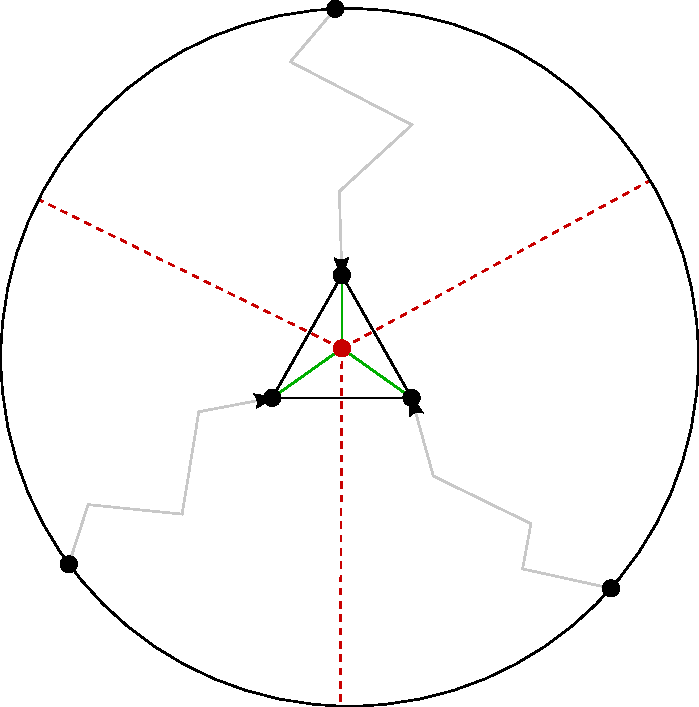
\includegraphics[width=0.66\textwidth]{figs/vd2.pdf}
  \caption{Illustration of $VD^*$ and a vertex in the graph. The vertex $v^*$ is given in
  red and vertices of $G$ are given in black. The edges of $VD^*$ are given by red dashed
  lines and the edges
of $G$ are black. The artificial edges with zero weight we add are given in green. The
shortest path from the sites of the adjacent Voronoi cells to the vertex adjacent to the
face corresponding to $v^*$ is given in grey.}
    \label{vd2}
\end{figure}
\noindent \\
\indent \textit{Query}. Depending on the case that $G$ falls under, we do the following for the
query $Q(v, \lambda)$: \\
\\
\textbf{Case 1:} Look up the distance in the hash table stored for $v$. \\
\textbf{Case 2:} The query is $Q(u,\lambda)$. If the size of the $\lambda$ is polynomial,
we can look up the distance stored the hash table for that label in $O(1)$ time.
Otherwise the size of $\lambda$ is $\varepsilon_2$ and we refer to the data structure
described above. Let $\mathcal{V}\subset V$ be the set of vertices with label $\lambda$.
For each $v\in \mathcal{V}$, we do the following:\\
When a region $R$ is split into two regions $P$ and $Q$ with a Jordan curve $C$, if
either $u$ or $v$ belongs to $C$, then we can look up the distance in $O(1)$ time since
we have stored all distances to and from boundary nodes. If both belong to the same
subregion, we go into that piece. The last case is when $u\in P$ and $v\in Q$. In this
case, we can locate which hole $h$ which contains $v$. Since we have stored the
additively weighted Voronoi diagram $VD^*(u,h)$, we perform a point location query to
determine the site which $v$ belongs to in $VD^*$. Note that
$VD^*$ is a tree, so the idea is to construct a centroid decomposition of $VD^*$. To locate the
Voronoi cell $v$ belongs to, it is sufficient to locate a terminal edge $e^*$ of $VD^*$, so that
$v$ is in one of the two Voronoi cells adjacent to it. Now consider a vertex $v^*$
adjacent to three sites. We can determine which site is closest to $v^*$ and if it is
left or right of the shortest path from $s_i$ to $v^*$ (using preorder numbers in the
shortest path tree). Say $s$ is the site closes to $v^*$, it is adjacent to two edges of
$VD^*$. Depending on the position of $v$ relative (left or right) to the shortest path,
we traverse one of the edges $e^*$. If $v$ is directly on the shortest path, we can
deduct it belongs to the Voronoi cell of $s$ (refer to Figure \ref{vd1}). We continue this approach until we find a
terminal edge $e^*$, from which we can tell which cell $v$ belongs to by comparing the
distances to both sites.

\begin{figure}[h!]
  \centering
  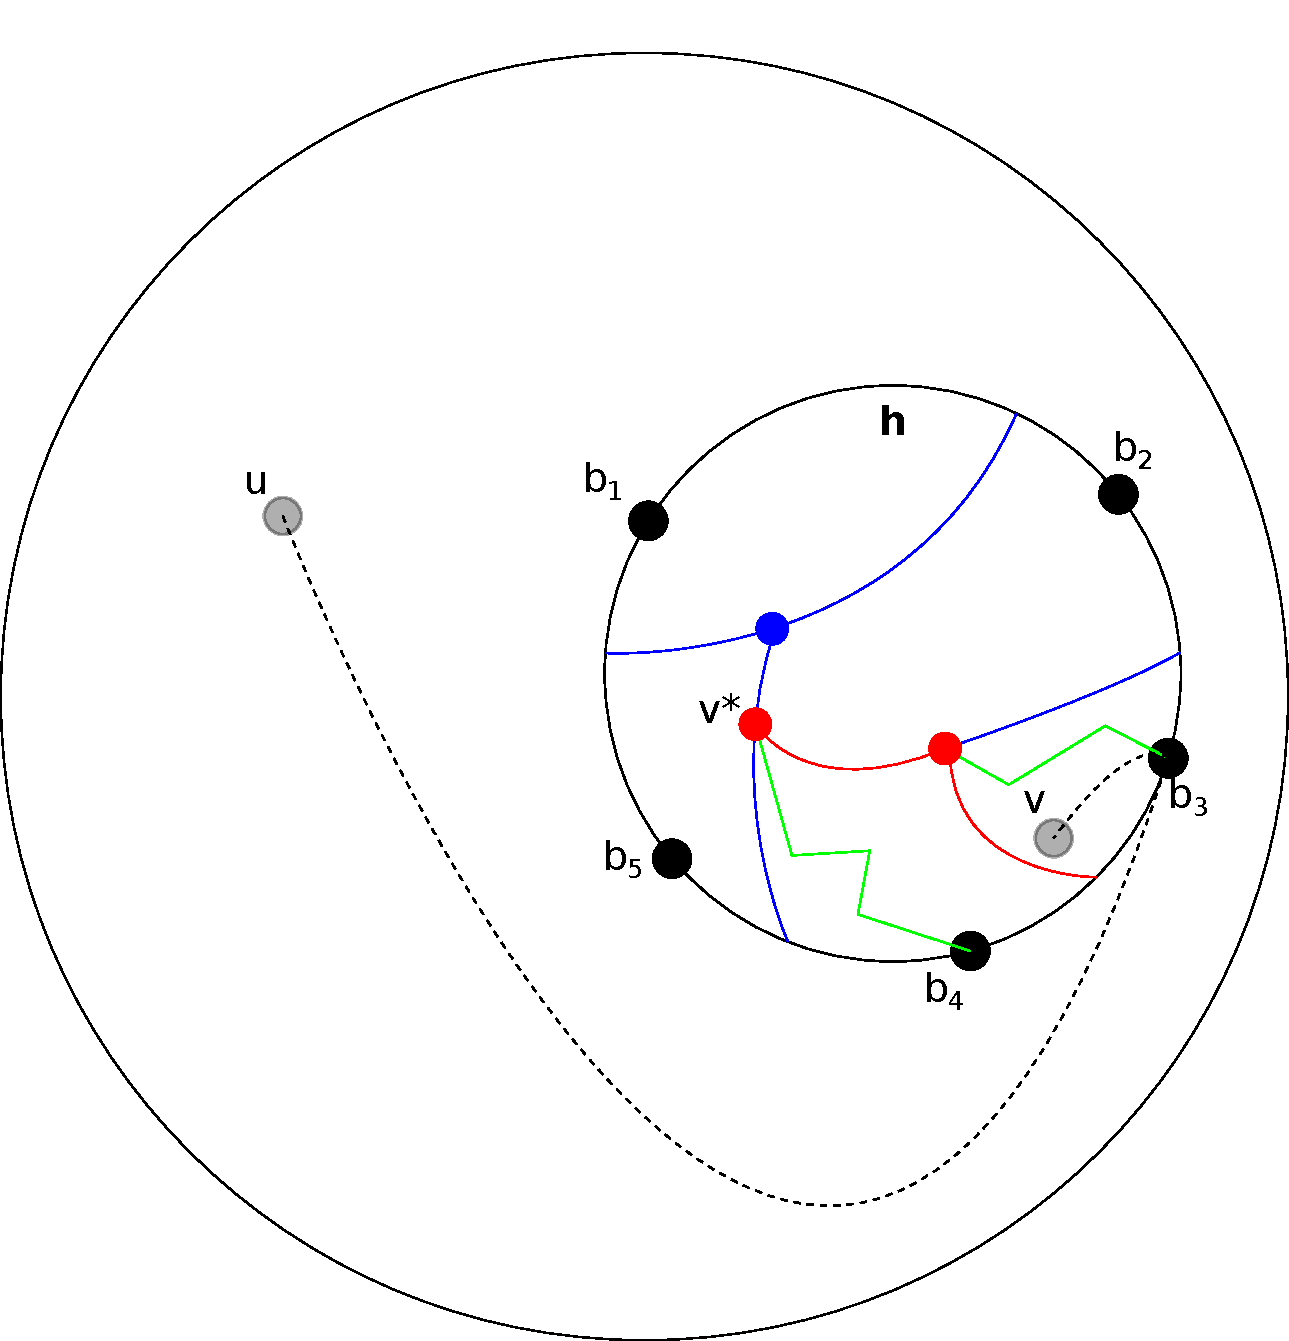
\includegraphics[width=0.66\textwidth]{figs/vd1.pdf}
  \caption{Illustration of how a query $Q(u,v)$ works. First, we determine which hole $v$
  belongs to (called P here). We then traverse our centroid decomposition of the
  additively weighted Voronoi diagram $VD^*(u,P)$ (in blue) starting at the vertex $v^*$ given in
red. We compare the distances from $u$ to $v$ through the three sites ($s_2$, $s_4$,
$s_5$). Say the shortest distance is through $s_4$, we need to locate $v$ relatively to
the shortest path from $s_4$ to $v^*$ (in green). Since $v$ is
located right of this path, we traverse the edge given in red. Again, we compare the
distances from $u$ to $v$ through the three sites $s_2$, $s_3$ and $s_4$. The shortest
path goes through $s_3$ and $v$ is located left of the shortest path from $s_3$ to the
Voronoi vertex, so again we traverse the corresponding edge. Since this is a terminal
edge, we can determine that $v$ belongs to the Voronoi cell of $s_3$.}
    \label{vd1}
\end{figure}

\subsubsection{Analysis}
\textbf{Preprocessing}.
In case 1, we need to store shortest path
trees from every node. Henzinger et al. showed that single source shortest paths can be
computed in $O(n)$ time \cite{henzinger1997faster} assuming non-negative edge lengths.
This means we can calculate the distance matrix in in $O(n^2)$, this
can be done in $O(n^{3/2})$ time. \\
In the other case, we need to preprocess it the same way, but we also need to compute
additively weighted Voronoi diagrams for every node $u\in P$ and hole $h$ of $Q$ when a
region is decomposed into two subregions. TODo \\
\\
\textbf{Space}.
In case 1, we store $\ell$ distances for each vertex $v$. Since $\ell=O(\sqrt{n})$, this
yields space $O(n^{3/2})$. \\
In case 2, since we assumed that there are no more that
$O(\sqrt{n})$ labels of size $\omega(\text{polylog}(n))$, the hash table storing the
distances to these labels cannot require more than $O(n^{3/2})$ space. The hash table
storing the size of all labels require $O(\ell)$ space. Additionally, every time we
separate the graph into $P$ and $Q$, we need to record whether vertices belong to $P$ or
$Q$ or the Jordan curve $C$. Since the recursive decomposition has depth $O(\lg n)$, the
space required for this is $O(\ell\lg n)$. \\
We also need to store all distances $\delta(u,v)$ and $\delta(v,u)$ for all
boundary vertices $u\in V$. Since the number of boundary vertices is $O(\sqrt{n})$, this
requires a total of $O(n^{3/2})$ space. \\
Lastly, we need to store additively weighted Voronoi diagrams for a vertex $u\in P$ and
hole $h$ of $Q$. Recall that we can store an additively weighted Voronoi diagrams in
$O(\sqrt{r})$. Since we store $O(1)$ diagrams (because each region has $O(1)$ holes) for
all vertices in the entire graph $G$, this requires a total space of $O(n\sqrt{r})$.
Thus the total space required is $O(n^{3/2}+\ell+\ell\lg n+n\sqrt{r})=O(n^{3/2})$. \\
\\
\textbf{Query}.
In case 1, we look up the distance in the hash table in $O(1)$ time.\\
In case 2, all labels have size $O(\text{polylog}(n))$. The point location method desribed
above takes $O(\lg n)$ time as we descend in the recursive decomposition with depth
$O(\lg n)$. Since the trees constructed for each additively weighted Voronoi diagram has
depth $O(\lg \sqrt{r})$ and $r<n$, this term doesn't add to the query time. However,
there can be up to $O(\text{polylog}(n))$ vertices of a given label, which means we have
to do $O(\text{polylog}(n))$ different point locations and extract the minimum. This
yields a total query time of $O(\text{polylog}(n))$. \\
\\
This gives us the distance oracle given in Theorem \ref{thm2}. \\
\\
TODO: Fix the gap ($\omega(\sqrt{n})$ labels with $\omega(\text{polylog}(n))$ size).
